\documentclass[11pt]{beamer}
\usepackage[utf8]{inputenc}
\usepackage[T1]{fontenc}
\usepackage{lmodern}
\usepackage[spanish]{babel}
\usepackage{amsmath}
\usepackage{hyperref}
\usepackage{amsfonts}
\usepackage{amssymb}
\usepackage{graphicx}
\usetheme{Frankfurt}
\usepackage{tikz}
\titlegraphic{\vspace{8cm}}% to push the other text to the top
\begin{document}
	\author{
		Departamento de Investigacion en F\'isica \\
		Maestría en Ciencias (Física)\\
		Hiram Ernesto Dami\'an}
	\title{Producción del bosón de Higgs en asociación con un solo quark de tipo top en colisiones protón-protón con el experimento CMS del CERN}
	%\subtitle{}
	\logo{
\includegraphics[scale=0.1]{unison-logo.png}}
	\institute{Universidad de Sonora}
	%\date{}
	%\subject{}
	\newcommand{\subf}[2]{%
		{\small\begin{tabular}[t]{@{}c@{}}
				#1\\#2
		\end{tabular}}%
	}
	%\setbeamercovered{transparent}
	%\setbeamertemplate{navigation symbols}{}
	\begin{frame}
	\titlepage
\end{frame}

\begin{frame}
\tableofcontents
\frametitle{Contenido}
\end{frame}

\begin{frame}
\section{Objetivo}
\subsection{Objetivo general}
\frametitle{Objetivo general}
\begin{itemize}
\item Mediante este proyecto se investigará la producción del bosón de Higgs en asociación
con un solo quark de tipo top (tH) en colisiones protón-protón con el experimento CMS
del LHC. Este mecanismo de producción del bosón de Higgs no ha sido observado antes
por ningún experimento.\\

\item El entender la producción del bosón de Higgs, así como sus
decaimientos son una parte importante del programa de física de los experimentos del
laboratorio internacional CERN que intenta completar las pruebas para verificar el
Modelo Estándar, la teoría de las partículas fundamentales.
\end{itemize}

\end{frame}


\begin{frame}
\frametitle{Modelo est\'andar}
\section{Antecedentes}
\subsection{Modelo est\'andar}
\begin{center}
\begin{figure}[ht]
	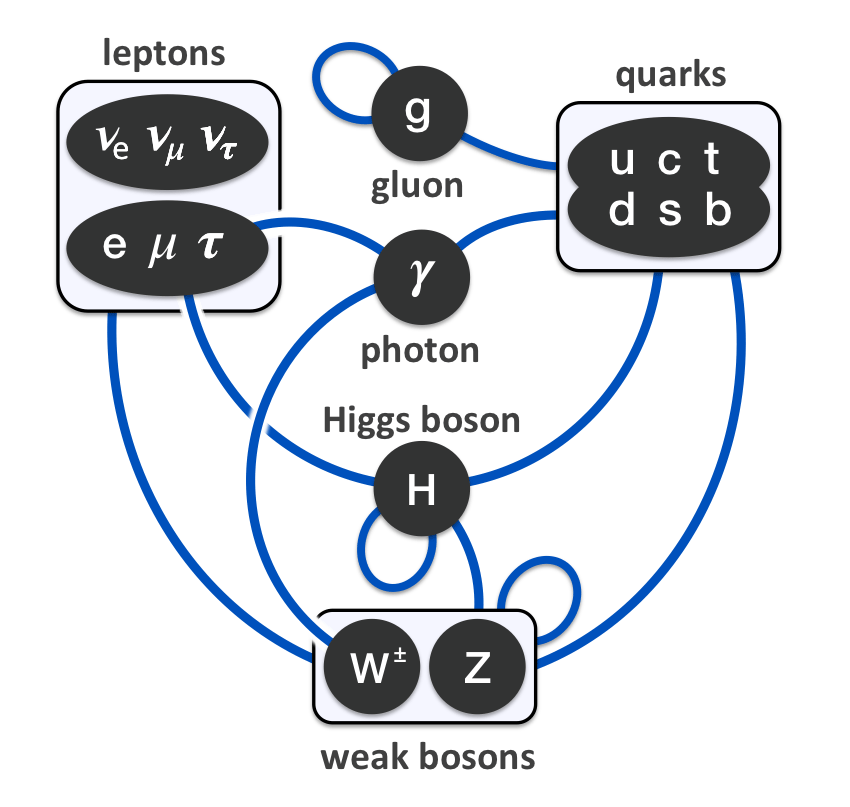
\includegraphics[scale=0.25]{sm.png}
\end{figure}
\end{center}
\end{frame}

\begin{frame}
\subsection{Descubrimiento del Higgs}
\frametitle{Descubrimiento del Higgs}
En 2012, las colaboraciones ATLAS y CMS anunciaron el descubrimiento de un nuevo bosón. Hasta ahora, todas las medidas de sus propiedades son consistentes con las del bosón de Higgs del modelo estándar (SM). 
Sin embargo, pequeñas desviaciones de las predicciones del SM podrían 
estar asociadas con física más allá del modelo estándar (BSM). \\

Las mediciones de alta  precisi\'on de las propiedades de este bos\'on son por tanto cruciales para responder a la pregunta de si la partícula encontrada es realmente consistente con la predicci\'on del SM.
\end{frame}


\begin{frame}
\frametitle{Detector CMS}
\begin{center}
\begin{figure}
	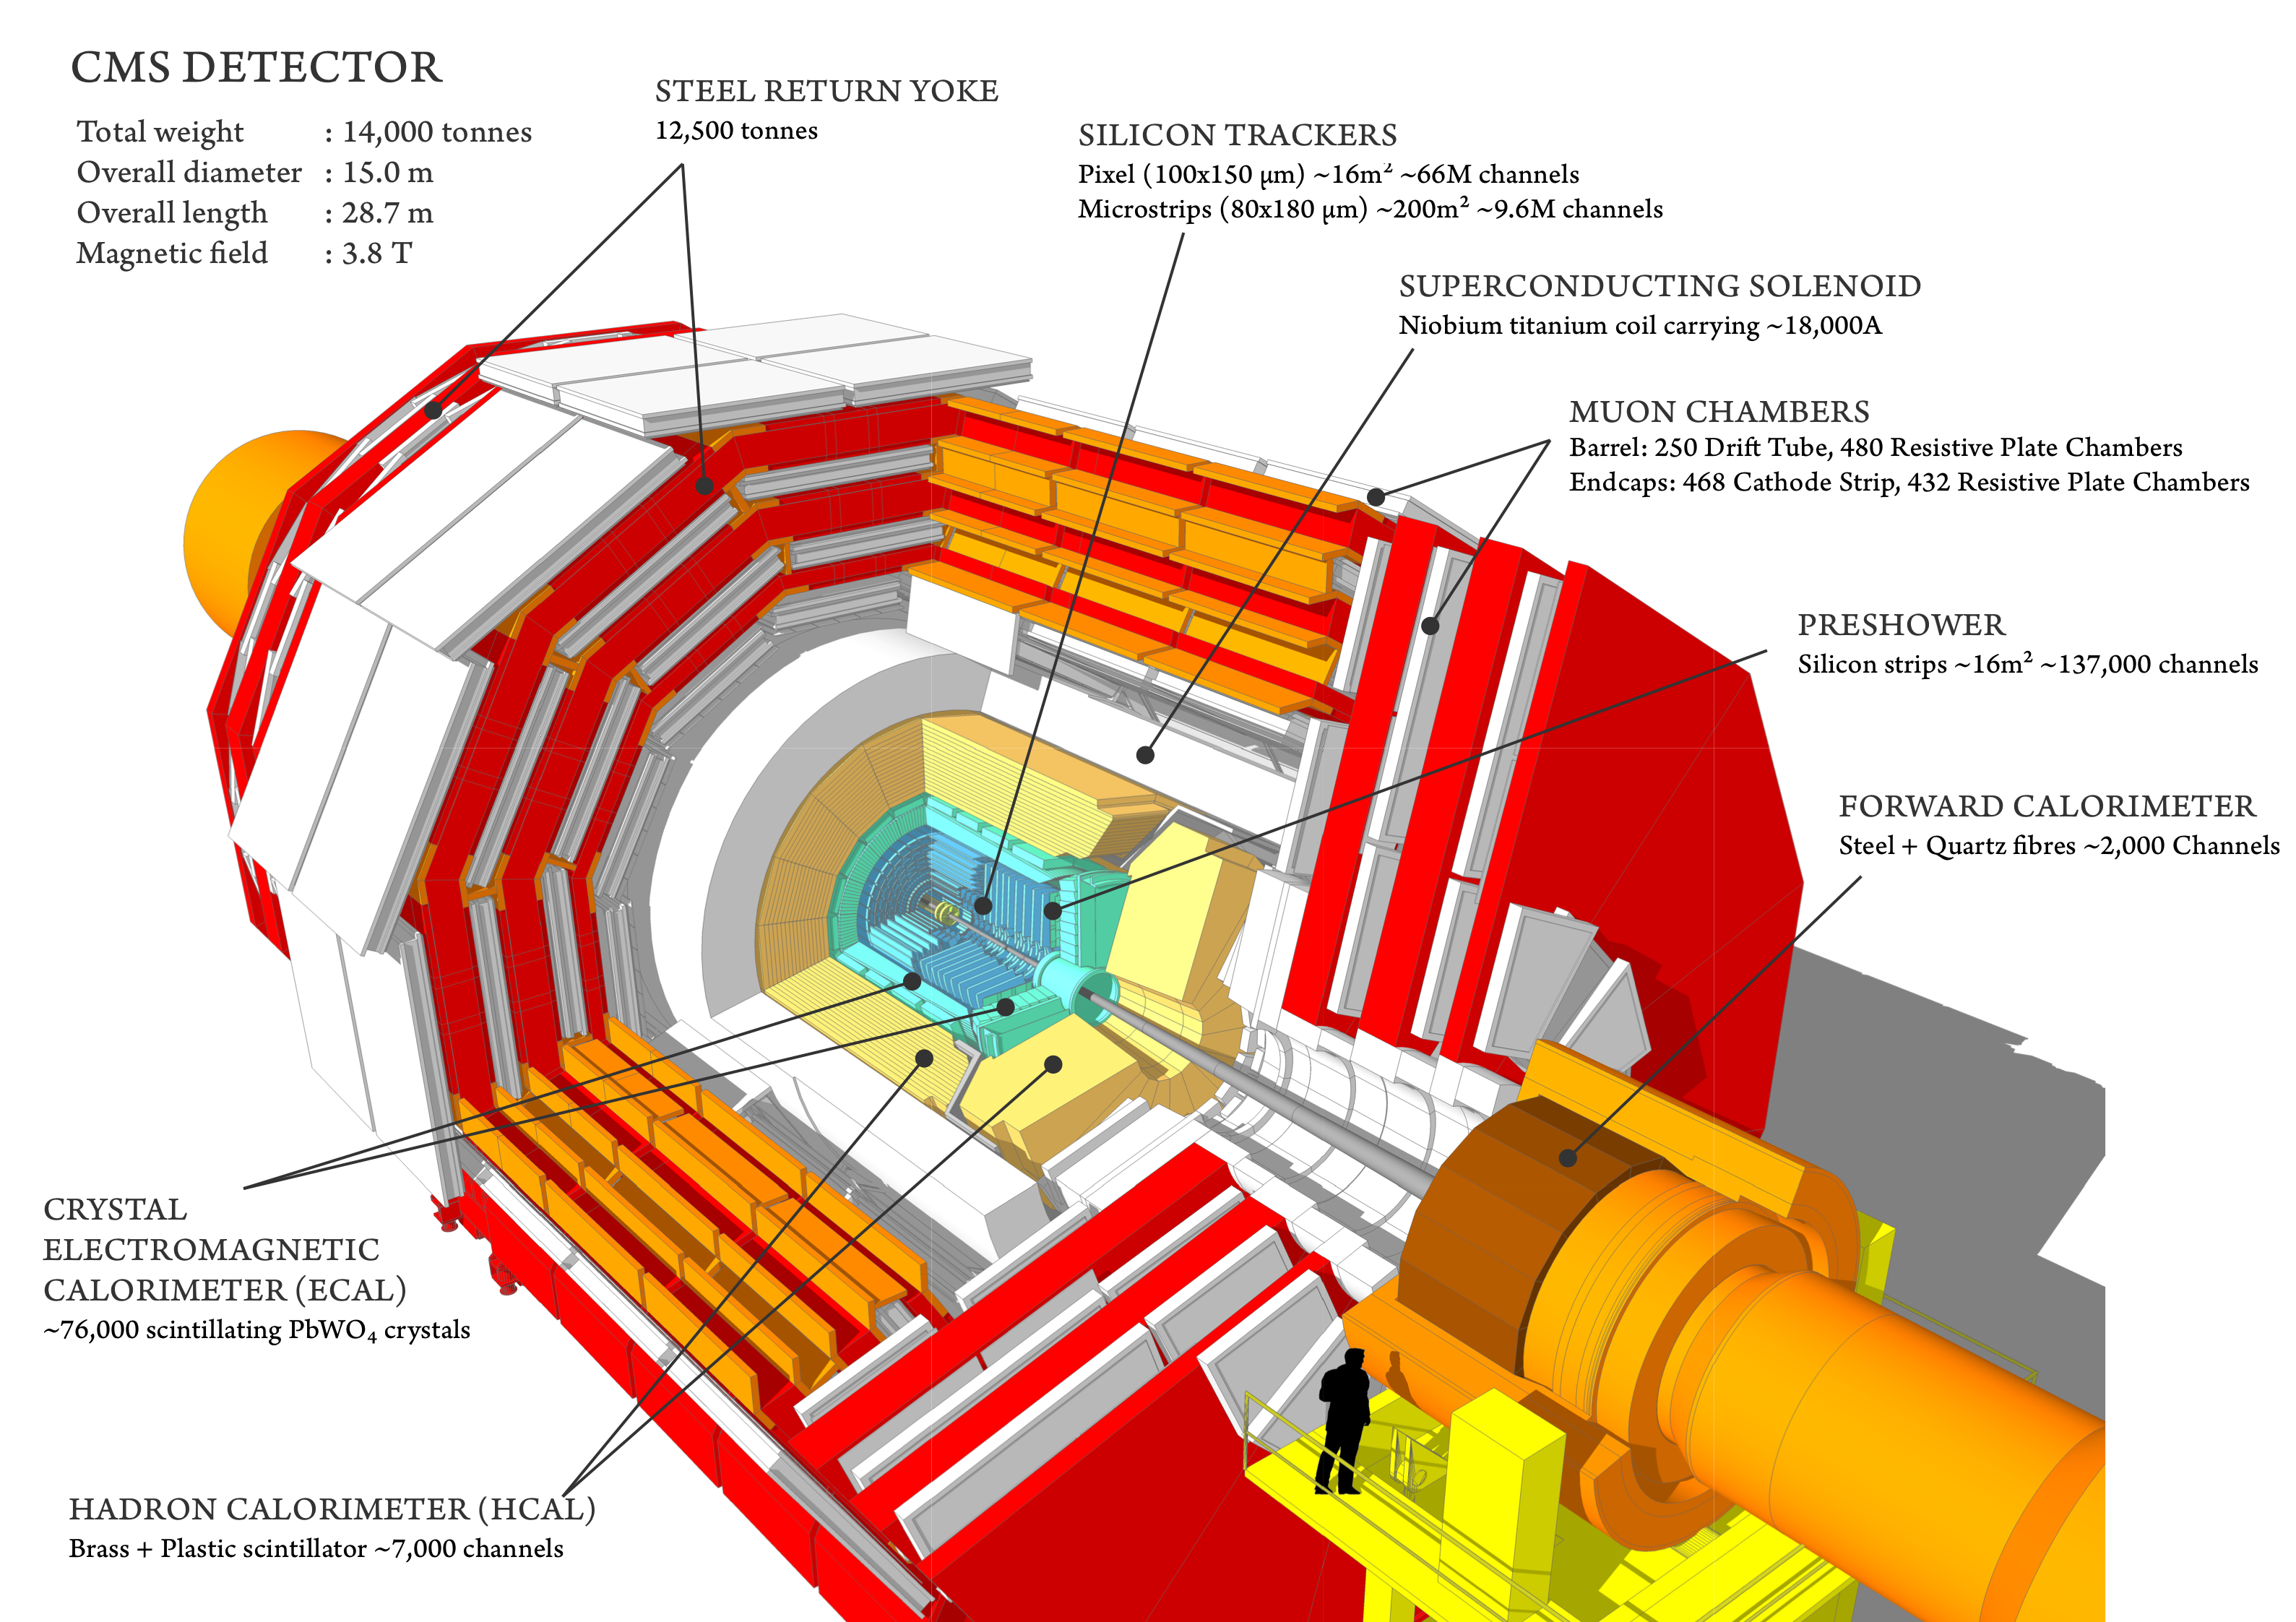
\includegraphics[width=\linewidth]{cms.png}
	\caption{Detector CMS del Cern (Lado franc\'es)}
\end{figure}
\end{center}
\end{frame}
\begin{frame}
\frametitle{Mecanismo de producci\'on}
\begin{center}
\begin{figure}
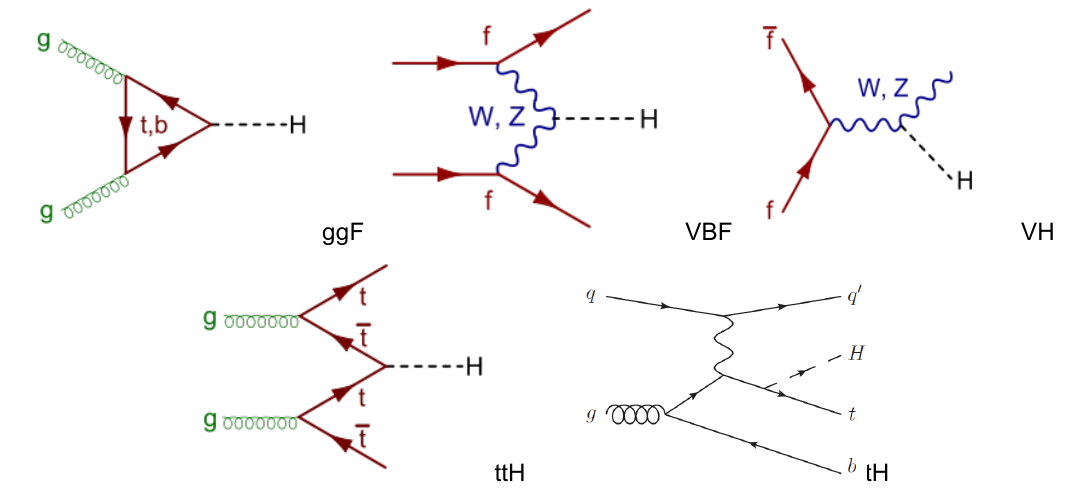
\includegraphics[width=\linewidth]{pg.png}
\caption{canales de producci\'on del bos\'on de Higgs}
\end{figure}
\end{center}
\end{frame}

\begin{frame}
\frametitle{Mecanismo de producci\'on}
\begin{center}
\begin{figure}
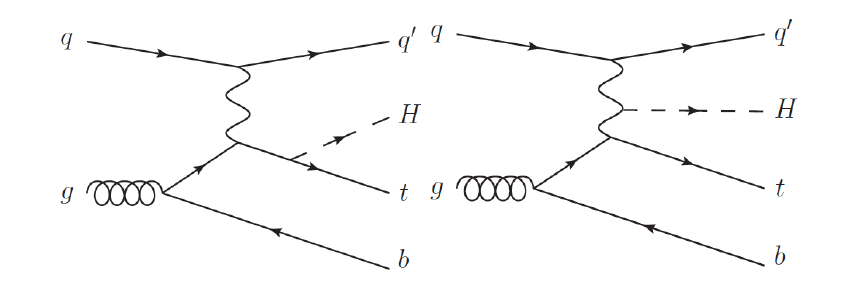
\includegraphics[width=\linewidth]{tq.png}
\caption{canales de producci\'on \textsc{tH}}
\end{figure}
\end{center}	
\end{frame}

\begin{frame}
\frametitle{Canales de producci\'on de Higgs}
\begin{center}
\begin{figure}
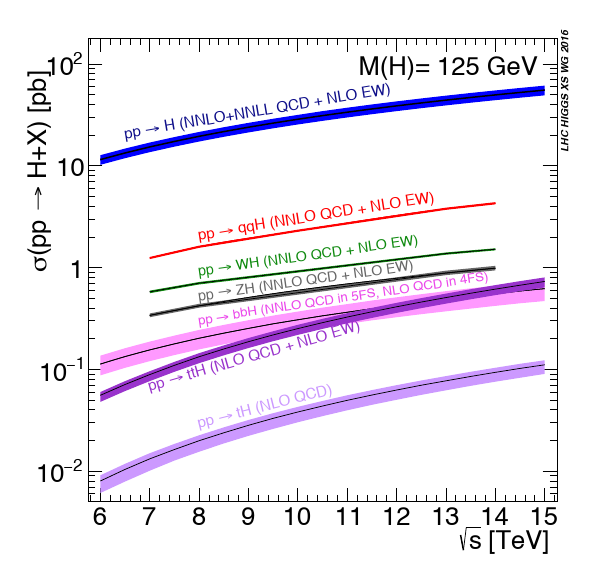
\includegraphics[scale=0.5]{yuk.png}
\end{figure}
\end{center}
\end{frame}




\begin{frame}
\section{Propuesta}
\frametitle{Propuesta}
En este proyecto se propone estudiar el bosón de Higgs en el proceso de producción de
tH con el experimento CMS del CERN. Para estos estudios se usarán los datos de la
segunda etapa de toma de datos 2 (2015-2018) del LHC y se espera también publicar proyecciones para la fase
de alta luminosidad del LHC (HL-LHC) que empezara en el 2026.

\end{frame}

\begin{frame}
\section{Justificaci\'on}
\frametitle{Justificación}
\begin{itemize}
\item Observación de proceso tH no antes visto.
\item El acoplamiento t-H (Yukawa top)  se puede medir en el proceso de producción ttH pero ese proceso no define el signo,  observación de tH define el signo.  
\end{itemize}
\end{frame}

\begin{frame}
\frametitle{Justificaci\'on}
	\begin{center}
		\begin{figure}
			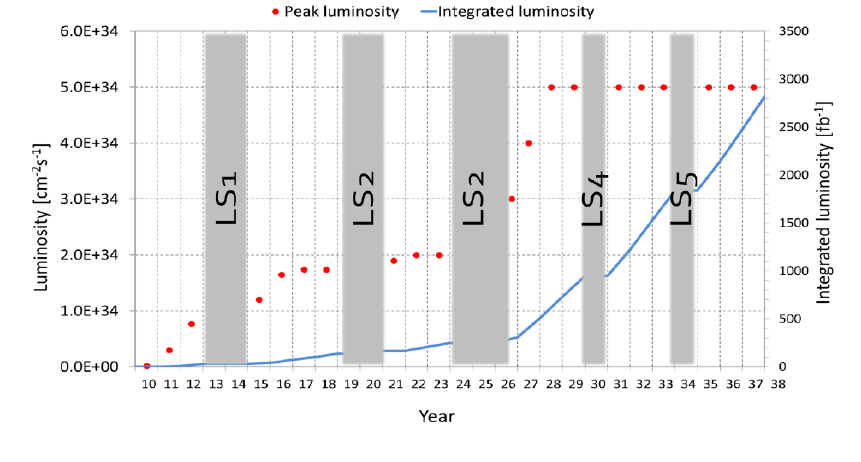
\includegraphics[width=\linewidth]{lum.png}
			\caption{ Rendimiento proyectado del LHC hasta 2038, que muestra las fechas
				preliminares para paradas prolongadas (LS) del LHC y luminosidades. Los puntos
				muestran la luminosidad instantánea mientras que la línea muestra la
				luminosidad acumulada.}
		\end{figure}
	\end{center}
\end{frame}


\begin{frame}
\subsection{Objetivos espec\'ificos}
\frametitle{Objetivos espec\'ificos}
Algunos de los objetivos en este proyecto incluyen:
\begin{itemize}
	\item verificar que la simulación de los eventos de señal sea adecuada,
	\item estudiar cual canal de decaimiento del bosón de Higgs es el mas \'optimo, hasta el
	momento se incluyen los canales ZZ, WW, par de leptones tau, y par de quarks b,
	\item estudiar aspectos en la reconstrucción que pueden mejorar la eficiencia, por
	ejemplo, las distribuciones de las partículas en el estado final del quark top,
	\item estudiar los ajustes para la extracción de la fuerza de la señal y su incertidumbre.
\end{itemize}
\end{frame}

\begin{frame}
\section{Metodolog\'ia}
\frametitle{Metodolog\'ia}
Los aspectos de la simulación de la producción de la señal se estudian a base de
generadores como MadGraph y Pythia que simulan las interacciones de los quarks y
gluones tomando en cuenta las distribuciones de probabilidad de cada tipo de partícula.\\

Estos son paquetes de software que se controlan con archivos de configuración que
definen varios aspectos como son los canales de decaimiento, la energía en el centro de
masa y afinamientos en el desarrollo de los jets que se generan por la interacción Fuerte
de los quarks.
\end{frame}

\begin{frame}
\frametitle{Metodolog\'ia}
\framesubtitle{Actualizaci\'on de datos}
Incorporar nuevos datos a un análisis requiere de algunos cuidados ya que la calibración
de los detectores y la reconstrucción de las partículas suele cambiar para cada periodo.
Es necesario entender cualquier cambio en la eficiencia de reconstrucción. Esto
generalmente se hace haciendo comparaciones de las diferentes distribuciones
cinemáticas con periodos anteriores.

\end{frame}

\begin{frame}
\frametitle{Metas}
\section{Metas}
\begin{itemize}
	\item Encontrar los canales de decaimiento del Higgs óptimos para búsqueda de tH.
	\item Estudiar mejoras en la reconstrucción de los eventos y mejoras que puedan
	ayudar a discernir tH y ttH.
	\item Incorporar los nuevos datos de CMS del 2017 y 2018 que mejoraran la
	sensibilidad.
	\item Mejorar los ajustes a los datos incluyendo nuevos datos y actualizando las
	incertidumbres sistemáticas.
	\item Estudiar la evolución de la sensibilidad a la señal de tH en función de la
	luminosidad acumulada en las diferentes fases del LHC.
\end{itemize}
\end{frame}

\begin{frame}
\section{Resultados}
\frametitle{Resultados esperados}
\begin{itemize}
 \item Generar los eventos de señal en al menos uno de los canales de decaimiento del
Higgs.
 \item Mejorar la eficiencia de reconstrucción de la señal.
\item Calcular los limites en la sección eficaz incorporando los nuevos datos de CMS
del 2017 y 2018.
\item Calcular proyecciones de la sensibilidad a la señal para las siguientes fases del
LHC.
\end{itemize}
\end{frame}




\begin{frame}
\frametitle{Habilidades que se desarrollar\'an}
- Aprender la física de las partículas fundamentales. \\
- Aprender a programar en lenguajes como c++, Python y la paqueter\'ia ROOT.\\
- Técnicas de análisis de datos como encontrar correlaciones.\\
- Utilizar cómputo de alto rendimiento.\\
- Hablar en público y en el idioma ingl\'es.
\end{frame}


\begin{frame}
\section{Plan de Trabajo}
\frametitle{Calendario de actividades}
\textbf{Verano 2018}
\begin{itemize}
\item Estudiar el modelo estándar, especialmente lo relacionado con el bosón de Higgs
\item Aprender el lenguaje de programación ROOT que es basado en c++.
\item Aprender los conceptos básicos del análisis de datos en ROOT y paquetes de
software para generar eventos de señal.
\end{itemize}
\end{frame}

\begin{frame}
\frametitle{Calendario de actividades}
\textbf{Semestre 2018-2}
\begin{itemize}
	\item Tomar curso optativo de análisis de datos.
	\item Estudiar técnicas de reconstrucción de eventos en CMS.
	\item Estudiar ajustes a los datos actuales y proyecciones para las diferentes fases del
	LHC.
\end{itemize}
\textbf{Semestre 2019-1}
\begin{itemize}
	\item Tomar segundo curso optativo de física de partículas
	\item  Terminar ajustes a los datos incluyendo datos del 2017 y 2018
	\item Escribir tesis
	\item Participación en congreso	
\end{itemize}
\end{frame}

\begin{frame}
\section{Avances recientes}
\frametitle{Avances recientes}
En el transcurso del mes, hemos realizado pr\'acticas de programaci\'on con ROOT, con el fin de familiarizarme con el ambiente.
Se ha trabajado con simulaciones de producci\'on de Higgs y generadores de eventos con pythia.
\end{frame}


\begin{frame}
\frametitle{Avances recientes}
\begin{figure}
	\centering
	\begin{tabular}{|c|c|}
		\hline
		\subf{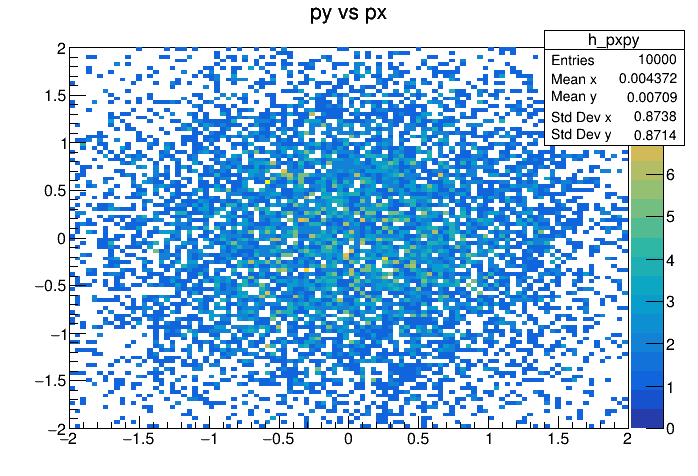
\includegraphics[width=40mm]{nou.png}}
		{}
		&
		\subf{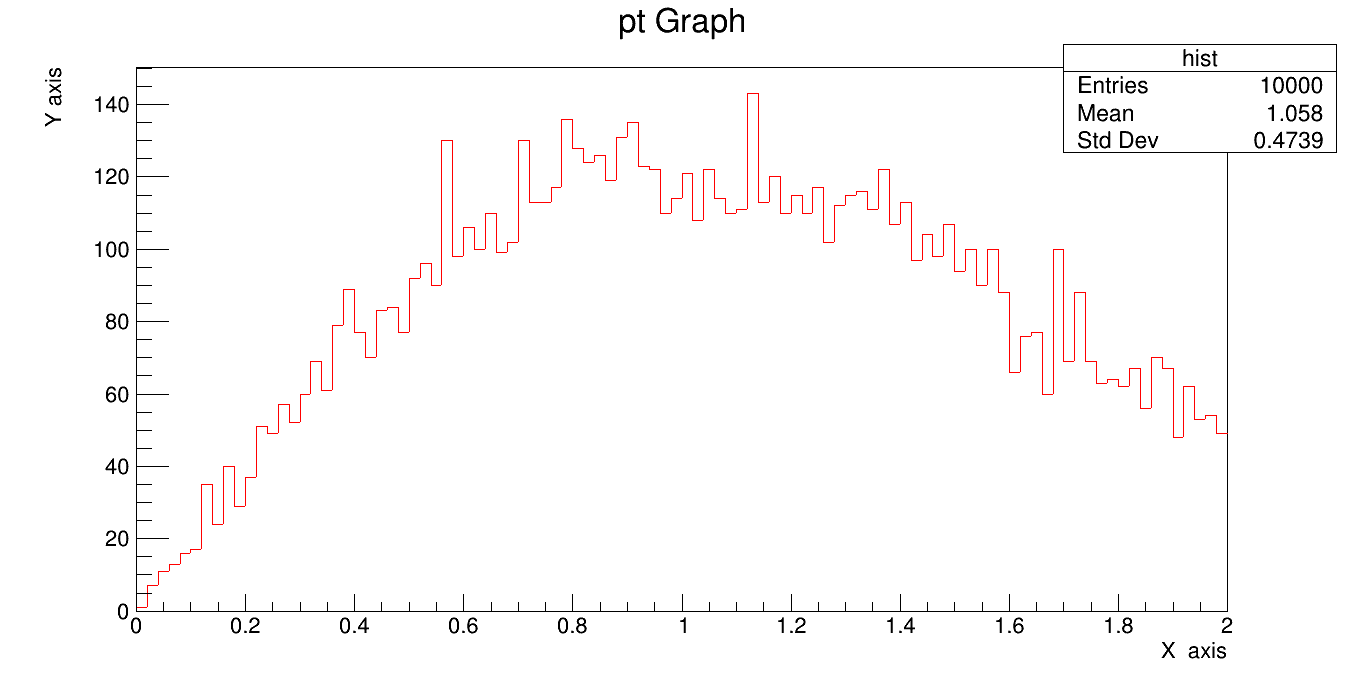
\includegraphics[width=40mm]{c1.png}}
		{}
		\\
		\hline
	\end{tabular}
\caption{Visualizaci\'on de eventos simulados con ROOT. \linebreak Gr\'aficas de momentos}
\end{figure}
\end{frame}

\begin{frame}
\section{Infraestructura y recursos }
\frametitle{Infraestructura y recursos}
\begin{itemize}
\item Acceso al clúster de computo \textsc{ACARUS} de la Unison y también remotamente a los centros
de computo de los laboratorios Fermilab y CERN.
\item El director de este proyecto esta actualmente aplicando a convocatorias de
CONACYT para conseguir fondos para movilidad.
\item Se colabora con grupos de investigación en los laboratorios Fermilab y CERN lo
cual permite hacer estancias en estos centros de investigación.
\item Posibilidad de presentar un trabajo en congresos nacionales o
internacionales.
\item Beca CONACYT.
\end{itemize}
\end{frame}


\begin{frame}
\section{Referencias}
\frametitle{Referencias}
\bibliographystyle{amsalpha}
\begin{thebibliography}{99}
%\bibitem{c1}The CMS collaboration, \"Observation of ttH production”, PRL 120 (2018) 231801
\bibitem{c5}\"Measurements of the Higgs boson production and decay rates and constraints on
its couplings from a combined ATLAS and CMS analysis of the LHC pp collision
data at $\sqrt{s}$ = 7 and 8 TeV”, J. High Energy Phys. 08 (2016) 045.
\bibitem{c2}The ATLAS Collaboration, \"Search for produced in association with top quarks
and constraints on the Yukawa coupling between the top quark and the Higgs
boson using data taken at 7 TeV and 8 TeV with the ATLAS detector “, Physics
Letters B 740 (2015) 222-242
\bibitem{c3}The CMS collaboration, \"Search for production of a Higgs boson and a single top
quark in multilepton final states in proton collisions at 13 TeV”, CMS-PAS-HIG-17-
005
\bibitem{c4}The CMS collaboration, \"Search for $H \rightarrow bb$ in association with a single top quark
as a test of Higgs boson couplings at $\sqrt{s}= 13$ TeV”, CMS-PAS-HIG-16-019
\end{thebibliography}
\end{frame}


\begin{frame}
\textsc{Gracias}
\end{frame}




\end{document}